\documentclass[8pt, landscape, a4paper]{extarticle}
\usepackage[top=0.2cm, bottom=0.2cm, left=0.2cm, right=0.2cm]{geometry}
\usepackage{amsmath, amssymb, amsfonts, bm, ctex, tikz, multicol}
\usetikzlibrary{shapes, arrows, positioning, calc}

% --- 极致紧凑格式设置 ---
\setlength{\parindent}{0pt}
\setlength{\parskip}{0pt}
\linespread{0.85} % 行间距压缩
\setlength{\columnsep}{0.2cm}
\setlength{\columnseprule}{0.1pt}
\pagestyle{empty}

% 压缩数学公式上下间距
\setlength{\abovedisplayskip}{1pt}
\setlength{\belowdisplayskip}{1pt}
\setlength{\jot}{0pt} 

% 自定义紧凑标题
\newcommand{\mysection}[1]{\vspace{1pt}\hrule\textbf{#1}\hrule}

% TikZ 全局样式缩小
\tikzset{
    block/.style={draw, rectangle, minimum height=1em, minimum width=1.5em, inner sep=1pt, font=\tiny},
    sum/.style={draw, circle, inner sep=0pt, minimum size=3mm},
    >=latex',
    every node/.style={font=\tiny}
}
\begin{document}

% 开始三栏布局
\begin{multicols*}{3} 

\section*{Lec1}

% 1. 微分方程与 Laplace 变换
$\ddot{y} \Rightarrow s^2 Y(s) - s y(0) - \dot{y}(0)$ \\[3pt]
$s \mathbf{X}(s) - \mathbf{x}(0) = \mathbf{AX}(s) + \mathbf{BU}(s)$ \\[5pt]

% 2. 极点与稳定性定义
$\lambda = \sigma + j\omega$ \hfill $\sigma$ --- Real part of pole --- stability \\
$e^{ts} = e^{\sigma t} e^{j\omega t}$ \hfill $\omega$ --- Imaginary part of pole --- oscillation \\[3pt]
{\footnotesize The unstable poles cannot be changed by the open loop control} \\[5pt]

% 3. 状态空间解与传递函数
$\mathbf{X}(s) = (s\mathbf{I} - \mathbf{A})^{-1} \mathbf{x}(0) + (s\mathbf{I} - \mathbf{A})^{-1} \mathbf{BU}(s)$ \\[3pt]
$H(s) = C(s\mathbf{I} - \mathbf{A})^{-1} \mathbf{b} = \frac{Q(s)}{P(s)}$ \\[3pt]
$P(s) = \det\{(s\mathbf{I} - \mathbf{A})\} = 0$ \\[5pt]

% 4. 反馈控制系统框图 (TikZ 实现)
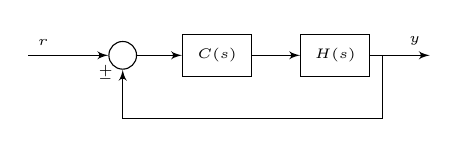
\begin{tikzpicture}[auto, node distance=1.2cm, >=latex']
    % 定义节点
    \node [coordinate] (input) {};
    \node [draw, circle, right of=input, inner sep=0pt, minimum size=10pt] (sum) {};
    \node [draw, rectangle, right of=sum, minimum height=1.5em, minimum width=2.5em] (controller) {$C(s)$};
    \node [draw, rectangle, right of=controller, node distance=1.5cm, minimum height=1.5em, minimum width=2.5em] (system) {$H(s)$};
    \node [coordinate, right of=system] (output) {};
    
    % 连接线
    \draw [->] (input) node[above right] {$r$} -- (sum);
    \draw [->] (sum) -- (controller);
    \draw [->] (controller) -- (system);
    \draw [->] (system) -- (output) node[above left] {$y$};
    
    % 反馈回路
    \draw [->] ($(system)!0.5!(output)$) -- ++(0,-0.8) -| node[pos=0.9, left] {$-$} (sum);
    \node at (sum) [below left] {\tiny $+$};
\end{tikzpicture}

% 5. 闭环传递函数
\vspace{3pt}
\[ \frac{Y(s)}{R(s)} = \frac{C(s)H(s)}{1 + C(s)H(s)} \]

% %%
% 请确保包含: \usepackage{amsmath, amsfonts, amssymb, ctex}

\section*{Lec2}

% 1. Z变换基本性质
$Z[x(k+1)] = zX(z) - zx(0)$ \\[3pt]
$Y(z) = y(0) + y(1)z^{-1} + y(2)z^{-2} + \dots$ \\[5pt]

% 2. 初值定理与终值定理
$f(0) = \lim_{s \to \infty} sF(s) \quad f(0) = \lim_{z \to \infty} F(z)$ \\[3pt]
$f(\infty) = \lim_{s \to 0} sF(s) \quad f(\infty) = \lim_{z \to 1} (z-1)F(z)$ \\[8pt]

% 3. 系统响应与稳态增益 (框图式描述)
$a^k \xrightarrow{\quad} \boxed{ H  } \xrightarrow{\quad} a^k H(a)$ \\[2pt]
{\scriptsize The static gain (the steady-state gain, or DC gain) --- $H(1)$} \\[2pt]
$C \xrightarrow{\quad} \boxed{ H } \xrightarrow{\quad} H(1)C$ \\[3pt]
$e^{st} \xrightarrow{\quad} \boxed{H(s)} \xrightarrow{\quad} e^{st} \xrightarrow{s=0} 1 \xrightarrow{\quad} \boxed{H} \xrightarrow{\quad} H(0) $\\[8pt]

% 4. 极点与零点映射关系 (中文说明)
极点: 有完美公式 $\lambda \to e^{\{\lambda h\}}$ 稳定的连续极点一定映射为稳定的离散极点。零点: 没有简单公式! \\[5pt]

% 5. 离散化公式 (采样)
$\Phi = e^{Ah}$ \\[3pt]
$\Gamma = (\int_0^h e^{A\tau} d\tau) b \quad F(s) = \mathcal{L}[f(t)] = (sI - A)^{-1}$ \\[5pt]

% 6. 算子定义与积分推导
$q f(k) = f(k+1) \quad \Gamma = \int_0^h e^{A\tau} d\tau B = A^{-1} e^{A\tau} \big|_{\tau = 0}^h B$ \\[3pt]
$q^{-1} f(k) = f(k-1) \quad = A^{-1}(e^{Ah}-I)B$ \\[8pt]

% 7. 离散状态空间解
$X(z) = (zI - \Phi)^{-1} zx(0) + (zI - \Phi)^{-1} \Gamma U(z)$

% 请确保包含: \usepackage{amsmath, amssymb}

\section*{Lec3}

% 1. 能控性矩阵与能观性矩阵 (位于第一栏左下角)
$W_c = \left[ \Gamma \quad \Phi\Gamma \quad \dots \quad \Phi^{n-1}\Gamma \right] \qquad 
W_o = \begin{bmatrix} C \\ C\Phi \\ \vdots \\ C\Phi^{n-1} \end{bmatrix}$ 
% Observable Canonical Form
\textbf{• Observable Canonical Form}

\[
x(k+1) = 
\begin{bmatrix} 
-a_1 & 1 & 0 & \dots & 0 \\ 
-a_2 & 0 & 1 & \dots & 0 \\ 
\vdots & \vdots & \vdots & \ddots & \vdots \\ 
-a_n & 0 & 0 & \dots & 0 
\end{bmatrix} x(k) + 
\begin{bmatrix} b_1 \\ b_2 \\ \vdots \\ b_n \end{bmatrix} u(k)
\]

\[
y(k) = \begin{bmatrix} 1 & 0 & \dots & 0 \end{bmatrix} x(k)
\]

\[
H(z) = \frac{b_1 z^{n-1} + b_2 z^{n-2} + \dots + b_n}{z^n + a_1 z^{n-1} + a_2 z^{n-2} + \dots + a_n}
\]

\vspace{10pt}

% Controllable Canonical Form
\textbf{• Controllable Canonical Form}

\[
z(k+1) = 
\begin{bmatrix} 
-a_1 & -a_2 & \dots & -a_n \\ 
1 & 0 & \dots & 0 \\ 
0 & 1 & \dots & 0 \\ 
\vdots & \vdots & \ddots & \vdots \\ 
0 & 0 & \dots & 0 
\end{bmatrix} z(k) + 
\begin{bmatrix} 1 \\ 0 \\ \vdots \\ 0 \end{bmatrix} u(k)
\]

\[
y(k) = \begin{bmatrix} b_1 & b_2 & \dots & b_n \end{bmatrix} z(k)
\]

% 关键:确保前面是垂直模式
\par
% \vspace{-18pt} % ← 调整这个值(-15 到 -22 之间通常合适)
\section*{Lec4}

\begin{minipage}{\linewidth}
\centering
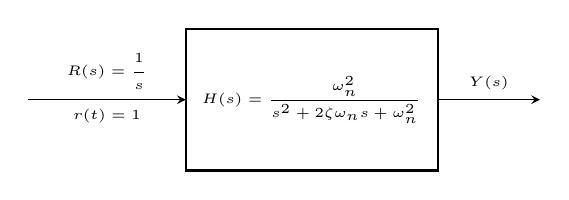
\begin{tikzpicture}[>=stealth, font=\small]
    % 输入信号线(带上下标注)
    \draw[->] (-2,0) -- (0,0);
    \node[above] at (-1,0) {$R(s) = \dfrac{1}{s}$};
    \node[below] at (-1,0) {$r(t) = 1$};
    
    % 传递函数框(加宽,单行 H(s))
    \draw[thick] (0,-0.9) rectangle (3.2,0.9);
    \node at (1.6,0) {$H(s) = \dfrac{\omega_n^2}{s^2 + 2\zeta\omega_n s + \omega_n^2}$};
    
    % 输出箭头
    \draw[->] (3.2,0) -- (4.5,0) node[midway, above] {$Y(s)$};
\end{tikzpicture}
\end{minipage}

\vspace{5pt}
\textbf{JURY'S STABILITY TEST:} \quad $A(z) = a_0 z^n + a_1 z^{n-1} + \dots + a_n = 0$ \\
\begin{tabular}{l l l l}
$1$ & $a_1$ & $a_2$ & \\
$a_2$ & $a_1$ & $1$ & $\times a_2$ \\ \hline
$1-a_2^2$ & $a_1(1-a_2)$ & & \\
$a_1(1-a_2)$ & $1-a_2^2$ & $\times \frac{a_1(1-a_2)}{1-a_2^2} = \frac{a_1}{1+a_2}$
\end{tabular}

\vspace{5pt}
\textbf{Controller:} \hfill $u(k) = -Lx(k) = -l_1 x_1(k) - l_2 x_2(k)$ \\
The closed-loop system: \hfill $x(k+1) = \Phi x(k) + \Gamma u(k) = (\Phi - \Gamma L)x(k)$ \\
\phantom{The closed-loop system:} \hfill $\Phi_{cl} \Rightarrow (\Phi - \Gamma L)$

\vspace{5pt}
$\mathcal{A}_m(z) = z^2 + p_1 z + p_2$ \\
① 算出 $|\lambda I - (\Phi - \Gamma L)|$, 得到含 $L$ 的多项式。 \\
令它等于参考多项式 $\mathcal{A}_m(z)$, 对比系数求解方程组 \\
\textbf{State-Feedback Controller:} \hfill $u(k) = -\tilde{L}z(k)$ \\
The closed-loop system: \hfill $z(k+1) = (\tilde{\Phi} - \tilde{\Gamma}\tilde{L})z(k) = (\tilde{\Phi} - \tilde{\Gamma}\tilde{L})z(k)$ \\
② 如果系统已经是可控标准型(第一行是非凡行) \\
$u(k) = -\tilde{L}z(k) = -[p_1 - a_1 \quad p_2 - a_2 \quad \dots \quad p_n - a_n]z(k)$

\vspace{5pt}
③ \textbf{Ackermann 公式 (通用神器)} \hfill $L = [0 \quad \dots \quad 0 \quad 1] W_c^{-1} \mathcal{A}_m(\Phi)$ \\
\textbf{deadbeat} \hfill $\mathcal{A}_m(z) = z^n \quad x(k+n) = (\Phi - \Gamma L)^n x(k) = 0$

\vspace{5pt}
\textbf{Observer Design} \\
$\hat{x}(k+1) = \Phi \hat{x}(k) + \Gamma u(k) + K(y(k) - \hat{y}(k))$ \\
$\hat{y}(k) = C\hat{x}(k)$ \\
$e(k+1) = \Phi e(k) - KCe(k) = (\Phi - KC)e(k)$ \\
$K = \mathcal{A}_o(\Phi) (W_o)^{-1} [0 \quad \dots \quad 0 \quad 1]^T$

\vspace{5pt}
Step 1: Controller Design \\
Step 2: Design observer to \\
estimate $x(k)$ \hfill $x(k+1) = \Phi x(k) + \Phi_{xw}\omega(k) + \Gamma u(k)$ \\
Step 3: $u(k) = -L\hat{x}(k)$ \hfill $\omega(k+1) = \Phi_\omega \omega(k)$ \\
Disturbance \hfill $y(k) = Cx(k)$



% 1. 带扰动模型的状态空间
\begin{minipage}{\linewidth}
$\begin{bmatrix} x(k+1) \\ \omega(k+1) \end{bmatrix} = \begin{bmatrix} \Phi & \Phi_{xw} \\ 0 & \Phi_\omega \end{bmatrix} \begin{bmatrix} x(k) \\ \omega(k) \end{bmatrix} + \begin{bmatrix} \Gamma \\ 0 \end{bmatrix} u(k)$ \\[5pt]
$y(k) = \begin{bmatrix} C & 0 \end{bmatrix} \begin{bmatrix} x(k) \\ \omega(k) \end{bmatrix}$ \\[8pt]

\hrule \vspace{3pt}
$L$ 和之前一样, $\hat{L} = \begin{bmatrix} L & L_\omega \end{bmatrix}$ \\[5pt]
$\begin{bmatrix} x(k+1) \\ \omega(k+1) \end{bmatrix} = \begin{bmatrix} \Phi - \Gamma L & \Phi_{xw} - \Gamma L_\omega \\ 0 & \Phi_\omega \end{bmatrix} \begin{bmatrix} x(k) \\ \omega(k) \end{bmatrix}$ \\[8pt]

\textbf{Ideal Case:} Choose $L_\omega$ such that $\Phi_{xw} - \Gamma L_\omega = 0$ \\
或常值 $w$: $H_\omega(1) = C[I - (\Phi - \Gamma L)]^{-1} (\Phi_{xw} - \Gamma L_\omega) = 0$
\end{minipage}

$\hat{z}(k+1) = \begin{bmatrix} \Phi & \Phi_{xw} \\ 0 & \Phi_\omega \end{bmatrix} \hat{z}(k) + \begin{bmatrix} \Gamma \\ 0 \end{bmatrix} u(k) + K(y(k) - \hat{y}(k))$ \\
$\hat{y}(k) = [C \quad 0] \hat{z}(k)$ \\
{\small $K$ can be chosen such that the C.P. of $(\hat{\Phi} - KC)$ matches any desired one.}

\vspace{5pt}
前馈 \\
$H_{ff} = L_c = \frac{B_m(z)}{B(z)}$ \\ $\frac{Y(z)}{U_c(z)} = H_{cl}(z) = L_c \frac{B(z)}{\mathcal{A}_m(z)} = \frac{B_m(z) B(z)}{B(z) \mathcal{A}_m(z)} = \frac{B_m(z)}{\mathcal{A}_m(z)} = H_m(z)$\\
$B(z)$ has to be stable for perfect tracking.

\section*{Lec5}% --- Lec5 RST 控制器部分 ---

\begin{center}
\begin{tikzpicture}[auto, node distance=2cm, >=Latex]

% --- 样式定义 ---
\tikzstyle{block} = [draw, rectangle, minimum height=2.5em, minimum width=3.5em]
\tikzstyle{sum} = [draw, circle, inner sep=0pt, minimum size=15pt]

% --- 坐标与节点定义 ---

% 1. 定义主水平参考线
\node [coordinate] (input_left) at (1.2,0) {}; % 左侧起点
\node [coordinate] (branch_point) at (3,0) {}; % 1/3 处的垂直分支点
\node [coordinate] (main_line_end) at (10,0) {}; % 右侧终点

% 2. 第一层:Reference Model (缩小宽度)
\node [block, right=0.2cm of branch_point, minimum width=2.5cm] (ref_model) {Reference Model $\frac{B_m(z)}{A_m(z)}$};
\node [coordinate, right=0.8cm of ref_model] (yr_out) {};

% 3. 第三层:反馈回路(主轴)
\node [sum] (sum1) at (1, -2.5) {};
\node [block, right=0.2cm of sum1] (S) {$\frac{S(z)}{R(z)}$};
\node [sum] (sum2) at (3, -2.5) {}; % 与 branch_point 垂直对齐
\node [block, right=0.2cm of sum2, minimum width=5em] (system) {System \hfill $\frac{B(z)}{A(z)}$};
\node [coordinate, right=1.2cm of system] (y_out) {};

% 4. 第二层:T(z)/R(z) 模块(精准对齐在 1/3 处)
\node [block, at={(3, -1.2)}] (T) {$\frac{T(z)}{R(z)}$};

% --- 连线绘制 ---

% 顶层 u_c 及其分支
\draw [-] (input_left) node[above right] {$u_c$} -- (branch_point);
\draw [->] (branch_point) -- (ref_model);
\draw [->] (branch_point) -- (T); % 垂直向下的第一条线
\fill (branch_point) circle (1.5pt);
\draw [->] (ref_model) -- (yr_out) node[above left] {$y_r$};

% 中间 T 模块到求和点
\draw [->] (T) -- node[right] {$u_{ff}$} (sum2); % 垂直向下的第二条线

% 底层主通道
\draw [->] (0, -2.5) -- node[pos=0.8, above] {$+$} (sum1);
\draw [->] (sum1) -- (S);
\draw [->] (S) -- node[above] {$u_p$} (sum2);
\draw [->] (sum2) -- node[above] {$u$} (system);
\draw [->] (system) -- (y_out) node[above left] {$y$};

% 反馈线
\draw [->] ($(system)!0.5!(y_out)$) -- ++(0,-1) -| node[pos=0.9, right] {$-$} (sum1);

% 干扰项
\node [coordinate, below=0.6cm of sum2] (dist_node) {};
\draw [->] (dist_node) node[right] {Disturbance $v$} -- (sum2);

% 求和点正号标注
\node at (sum2.west) [below left] {$+$};
\node at (sum2.north) [below left] {$+$};
\node at (sum2.south) [above right] {$+$};

% 底部文本
\node[below=1.2cm of S, xshift=1.2cm] {The simplest case: \hspace{1cm} $A(z)Y(z) = B(z)(U(z)+V(z))$};

\end{tikzpicture}
\end{center}

% {\footnotesize The simplest case: \hfill $A(z)Y(z) = B(z)(U(z) + V(z))$} \\[3pt]
$\frac{Y(z)}{U_c(z)} = \frac{T(z)B(z)}{A(z)R(z) + B(z)S(z)} = \frac{B_m(z)}{A_m(z)}$ \\[5pt]

\textbf{Back} \hfill $A_{cl}(z) = A(z)R(z) + B(z)S(z) = A_m(z) A_o(z)$ \\[5pt]
\textbf{Forward} \hfill $T(z) = t_0 A_o(z)$ \hfill  $T(z) = \frac{A_o(z)B_m(z)}{B(z)}$ \\[5pt]

如果系统阶数为 $n$ 则控制器 $Rz$ 和 $Sz$ 的阶数通常选为 $n-1$ \\
$A_o$ 补次数 $A_0=z$ \\
降维找稳定零点/极点, 从 TRS 里找 \\
干扰 \hfill $R = (z-1)R'(z)$
% 第二张图右下角:增量式状态空间模型
\textbf{干扰} \hfill $R = (z-1) R'(z)$ \\[5pt]
$x_p(k+1) = A_p x_p(k) + B_p u(k)$ \\
$y(k) = C_p x_p(k)$ \\[10pt]

\[
\overbrace{
  \begin{bmatrix}
    \Delta x_p(k+1) \\
    y(k+1)
  \end{bmatrix}
}^{z(k+1)}
=
\overbrace{
  \begin{bmatrix}
    A_p & 0 \\
    C_p A_p & 1
  \end{bmatrix}
}^{A}
\overbrace{
  \begin{bmatrix}
    \Delta x_p(k) \\
    y(k)
  \end{bmatrix}
}^{z(k)}
+
\overbrace{
  \begin{bmatrix}
    B_p \\
    C_p B_p
  \end{bmatrix}
}^{B}
\Delta u(k)
\]

\[
y(k) = 
\overbrace{
  \begin{bmatrix}
    0 & 1
  \end{bmatrix}
}^{C}
\,
\overbrace{
  \begin{bmatrix}
    \Delta x_p(k) \\
    y(k)
  \end{bmatrix}
}^{z(k)}
\]

\end{multicols*}

\end{document}